% Section 8.3: 3D accuracy against the simulator's trajectory log. Method: sections/reconstruction.tex (Section 5).
% Figures and numbers: writeup/make_camera_figures.py -> report/figures/camera/, writeup/figures/camera/stats.json

\subsection{3D Accuracy}
\label{sec:eval-3d}

Two recordings of one session (6,644 frames with the tip well inside the eye circle) were evaluated against the trajectory log. The reconstruction uses the calibration, including the eye roll, from the other recording; each recording's own
camera fit only aligns its log with the video in time and space and supplies the projections for frame selection and
the ideal input.

Two inputs are compared: (a) \emph{ideal}, the
logged tip and its modelled shadow projected into the image, which isolates the reconstruction but shares its
assumptions and so favours the perspective model; and (b) \emph{detected}, the segmenter's output as in live
operation.

\begin{table}[!htb]
  \centering
  \caption{3D tip error in mm, both recordings: median (range of the per-recording medians) and 95th percentile;
    height bias = median height error; found = share of frames with a 3D result; errors cover those frames only.}
  \label{tab:camera-accuracy}
  \small
  \begin{tabular}{llrrrr}
    \toprule
    input & camera model & median & p95 & height bias & found \\
    \midrule
    (a) ideal    & orthographic (eye circle)   & 1.95 (1.92--2.01) & 10.9 & $-0.79$ & 100\,\% \\
                 & perspective                 & \textbf{0.14} (0.12--0.14) & 0.51 & $-0.04$ & 100\,\% \\
    \midrule
    (b) detected & orthographic (eye circle)   & 1.62 (1.45--1.78) & 9.3  & $-0.48$ & 63\,\% \\
                 & perspective                 & \textbf{0.14} (0.12--0.14) & 0.64 & $-0.01$ & 67\,\% \\
    \bottomrule
  \end{tabular}
\end{table}

The perspective model reduces the median error by an order of magnitude with both inputs. With detected input, 97\,\% of the perspective results are within 1\,mm.

Most missing results are frames in which the segmenter did not find all four points (two jaw tips, two shadows); of
the frames with complete detections, the reconstruction itself rejects 43 with the perspective and 316 with the
orthographic model.

Figure~\ref{fig:camera-height} compares reconstructed and true height, the quantity that matters for guidance. The perspective model
follows the true height (median absolute error 0.07\,mm); the orthographic model scatters widely, mostly too low, and in 6\,\% of its results places the tip behind the retina.

In 3\,\% of the perspective results the height is off by more than 1\,mm, in 136 of 140 too low, i.e.\ closer to the
retina: there the detected shadow lies much closer to the tip in the image than the modelled one, so tip and shadow
appear to touch; in 36 of these frames the modelled shadow falls outside the visible eye circle.

\begin{figure}[!htb]
  \centering
  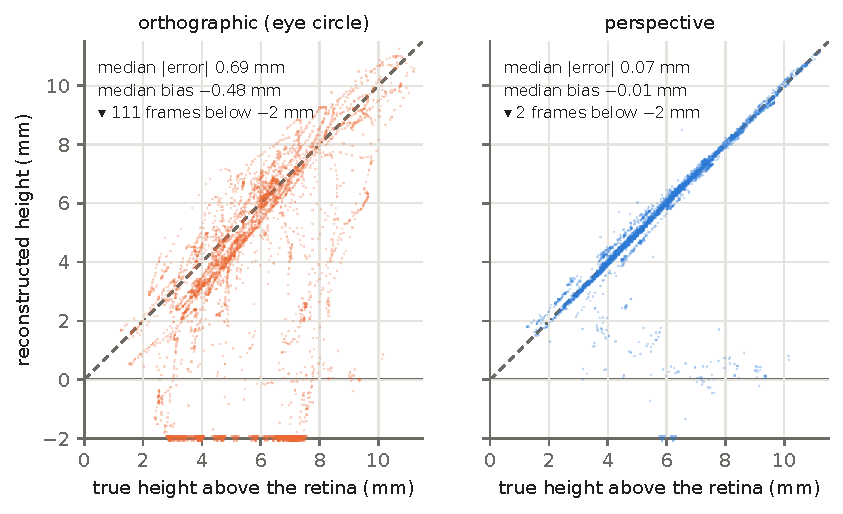
\includegraphics[width=0.8\linewidth]{figures/camera/height_error.pdf}
  \caption{Reconstructed against true height above the retina, detected input, one dot per frame with a 3D result.
    Dashed: reconstructed = true height. Triangles: reconstructed heights beyond the vertical range.}
  \label{fig:camera-height}
\end{figure}

A calibration from the evaluated recording itself changes the median by at most 0.04\,mm, while a 5$^\circ$ error in
the eye roll roughly doubles it.

The calibration needs the trajectory log and assumes a fixed light pipe.
